\documentclass[a4paper,12pt]{memoir}

\newsavebox{\FrontImgBox}
\newlength{\FrontClip}

\usepackage{float}
\usepackage[pdftex]{graphicx}
\usepackage{eso-pic}

% ====== A4 page layout ======
\settypeblocksize{*}{150mm}{1.6}
\setlrmarginsandblock{25mm}{25mm}{*}
\setulmarginsandblock{25mm}{25mm}{*}
\checkandfixthelayout
\usepackage{todonotes}
\pagestyle{empty} % no page number
\usepackage[pdftex]{graphicx}
\usepackage{eso-pic}

 \usepackage{microtype} % better justification & protrusion
\usepackage{newtxtext} % Times-like body text (newspaper vibe)
\usepackage[scaled]{helvet} % Sans for headlines and decks
\usepackage[T1]{fontenc}
\usepackage[utf8]{inputenc}
\usepackage{tikz}
\usetikzlibrary{decorations.text}

% ====== Columns & visuals ======
\usepackage{multicol}
\setlength{\columnsep}{0.28in}
\setlength{\columnseprule}{0.2pt}

\usepackage{graphicx}
\usepackage{wrapfig}
\usepackage{caption}
\captionsetup{font=small,labelfont=bf}

\usepackage[dvipsnames]{xcolor}
\usepackage{lettrine} % drop caps
\usepackage[many]{tcolorbox} % pull quotes / sidebars
%\usepackage[print,1to1]{booklet} %print option switches to landscape
%\pagespersignature{16}
\usepackage{pgfplots}
\pgfplotsset{width=10cm,compat=1.9}

\tcbset{
  colback=black!2,
  colframe=black!40,
  boxsep=4pt, left=6pt, right=6pt, top=6pt, bottom=6pt,
  sharp corners,
}

\usepackage{caption}
\captionsetup[figure]{labelformat=empty}

% ====== Headings & bylines ======
\setsecheadstyle{\Large\bfseries\sffamily}
\setsubsecheadstyle{\normalsize\bfseries\sffamily}
\setsubsubsecheadstyle{\normalsize\itshape}

\newcommand{\kicker}[1]{\textsf{\bfseries\small\color{Gray} #1}}
\newcommand{\headline}[1]{\textsf{\bfseries\fontsize{34}{36}\selectfont #1}}
\newcommand{\deck}[1]{\textsf{\large\itshape #1}}
\newcommand{\byline}[1]{\textsf{\small\color{Gray} Af #1}}
\usepackage{tikz}
\usetikzlibrary{fadings,patterns}

% Define a generic "fade to transparent" around a rectangle
\tikzfading[name=image fade,
  inner color=transparent!50,
  outer color=transparent!100]

  % Text outline ("border around letters")
\usepackage{contour} % works with pdfLaTeX/XeLaTeX/LuaLaTeX
\contourlength{0.9pt}         % default stroke thickness
\contournumber{32}            % smoothness of the outline

% Helpers: white text with dark outline (and a thinner variant)
\newcommand{\ow}[2][black]{\contour{#1}{\textcolor{white}{#2}}}
\newcommand{\owthin}[2][black]{%
  \begingroup\contourlength{0.6pt}\contour{#1}{\textcolor{white}{#2}}\endgroup}

% ====== Page banner / folio ======
\makepagestyle{newspaper}
\makeoddhead{newspaper}{\textsf{\small Den Rullende Sten}}{}{\textsf{\small Sponsoreret af Det Glemte Akademi}}
\makeevenhead{newspaper}{\textsf{\small Sponsoreret af Det Glemte Akademi}}{}{\textsf{\small Den Rullende Sten}}
\makeoddfoot{newspaper}{}{\textsf{\small\thepage}}{}
\makeevenfoot{newspaper}{}{\textsf{\small\thepage}}{}
\makeheadrule{newspaper}{\textwidth}{0.4pt}
\pagestyle{newspaper}

% ====== Pull quote and sidebar environments ======
\newenvironment{pullquote}
  {\begin{tcolorbox}[enhanced, breakable]\itshape\large}
  {\end{tcolorbox}}


\usepackage{xparse}
\usepackage{wrapfig}

% Justérbare standarder for sidebar i spalter
\newcounter{sidebarlines}              % hvor mange linjer der skal "wrappe" forbi boksen
\setcounter{sidebarlines}{14}
\setlength{\sidebarwidth}{0.42\columnwidth}

\newcommand{\godentry}[5]{%
% #1 = placering, #2 = titel, #3 = billedfil, #4 = side l/r, #5 = tekst
\begin{wrapfigure}{#4}{0.24\columnwidth}
  \vspace{-8pt}
  \centering
  \includegraphics[width=0.20\columnwidth]{#3}
  \vspace{-12pt}
\end{wrapfigure}

\subsection*{#1. #2}
#5

\par\medskip
}

% ====== Utilities ======
\newcommand{\separator}{%
  \par\noindent{\color{black!40}\rule{\textwidth}{0.4pt}}\par
}


% Front feature image: spans \textwidth, keeps aspect ratio, fades at edges,
% and overlays outlined text (no boxes).
% Usage: \FrontFeatureImage{<image>}{<kicker>}{<headline>}{<deck>}{<credit>}
\newcommand{\FrontFeatureImage}[5]{%
  % Typeset image at \textwidth just once and measure its height
  \sbox{\FrontImgBox}{\includegraphics[width=\textwidth]{#1}}%
  % Total height of the scaled image (height + depth)
  \dimen0=\dimexpr\ht\FrontImgBox+\dp\FrontImgBox\relax
  % Max allowed height
  \dimen2=.75\textheight
  % Choose visible height: min(actual, max)
  \ifdim\dimen0>\dimen2
    \setlength{\FrontClip}{\dimen2}%
  \else
    \setlength{\FrontClip}{\dimen0}%
  \fi
  %
  \begin{tikzpicture}
    % Define a "frame" we’ll use for anchors & clipping
    \coordinate (TL) at (0,0);                       % top-left
    \coordinate (TR) at (\textwidth,0);              % top-right
    \coordinate (BL) at (0,-\FrontClip);             % bottom-left (cropped)
    \coordinate (BR) at (\textwidth,-\FrontClip);    % bottom-right (cropped)

    % Image with soft fading edges, clipped to the frame (crops from the bottom)
    \begin{scope}
      \clip (TL) rectangle (BR);
      \node[anchor=north west, inner sep=0pt,
            path fading=image fade, fit fading=false] at (TL)
        {\usebox{\FrontImgBox}};
    \end{scope}

    % Dark wash for legibility, also softly faded (match the same clip)
    \begin{scope}
      \clip (TL) rectangle (BR);
      \fill[black,opacity=0.30, path fading=image fade] (BL) rectangle (TR);
    \end{scope}

    % Text stack (bottom-left) — outline style preserved
    \node[anchor=south west, xshift=1em, yshift=1em, align=left,
          text width=.75\textwidth] at (BL){%
      \sffamily
      % Kicker (optional)
      \if\relax\detokenize{#2}\relax\else
        {\owthin[black!85]{\textsf{\bfseries\small #2}}}\\[0.15em]\fi
      % Headline
      {\ow{\bfseries
        \resizebox{1\textwidth}{!}{#3}%
      }}\\[0.2em]
      % Deck
      {\owthin{\large\itshape #4}}%
    };

    % Credit (bottom-right), small outline
    \node[anchor=south east, xshift=-1em, yshift=1em] at (BR)
      {\sffamily\small \owthin[black!85]{#5}};
  \end{tikzpicture}%
}



 

\begin{document}
%\pdfpageheight=\paperwidth
%\pdfpagewidth=\paperheight
%\paperwidth=\pdfpagewidth
%\paperheight=\pdfpageheight 
% ====== Nameplate ======
\begin{figure}
  \begin{center}
      
\includegraphics[width=0.98\textwidth]{Logo.png}%
  \end{center}    
\end{figure}
\begin{center}
  {\Large\sffamily Udgave 132}
\end{center}


% Front feature image (keeps aspect ratio, spans \textwidth)
\FrontFeatureImage{DæmonAngreb.png}
{A'kastin er reddet!}
{KELLWAN KIRKEN SEJRE!}
{Endnu en sejer}
{}

\vspace{.75\baselineskip}
\newpage

% ====== Lead story (Front page) ======
\par\medskip
\headline{Kelllwan Kirken bygger Sydporten}
\par\medskip
\deck{A'kastin i evig gæld til Kelllwan Kirken}
\par\medskip
\byline{Redaktionen}
\medskip

\lettrine[lines=3,lhang=0.1,loversize=0.05]{D}{et} har længe været en kilde til både bekymring og debat: forbindelsen mellem A'kastin og det ødelagte land Letho. Nu melder Kelllwan Kirken sig på banen med et klart budskab. Arbejdet med Sydporten er endelig i gang.

\par\medskip

Efter flere mislykkede forsøg fra lokale kræfter i A'kastin på at sikre grænsen, har Kelllwan Kirken under ledelse af Sølvhammeren Orden påbegyndt en rekonstruktion af den længe omtalte port. Kirken beskriver selv indsatsen som både nødvendig og rettidig, og flere af deres repræsentanter fremhæver, at projektet allerede viser tegn på “struktur og disciplin, som tidligere har manglet.”

\par\medskip

Ifølge kirken er det særligt Sølvhammerens Orden, der har været afgørende for, at arbejdet overhovedet kunne begynde. Deres tilstedeværelse i A'kastin er blevet præsenteret som et vendepunkt, hvor tidligere kaotiske forsøg nu erstattes af en mere organiseret indsats.

\par\medskip

Flere talspersoner fra Kelllwan Kirken har udtalt, at hjælpen fra Dorian Vinterkrone også har været værdsat. De peger på, at A'kastin i årevis har stået over for trusler fra Letho uden at formå at etablere en holdbar løsning, og det var Dorian Vinterkrone som lod Sølvhammerens Orden gøre de nødvendige handlinger. Med rekonstruktionen af Sydporten mener kirken, at en sådan løsning nu er inden for rækkevidde.

\begin{pullquote}
“Det er ikke nok at erkende problemet. Man må også have evnen til at handle på det. At direktøren for Handelskompagniet kommer og tager æren virker dog som klassisk grådighed, da Handelskompagniet nægtede en fælles løsning, og alt betaling kom direkte fra direktørens egen lomme.”
- Biskop Edward Valmund 
\end{pullquote}

\par\medskip

Kelllwan kirken fremhævede især den manglende hjælp fra andre kirker og organisationer, her blev især fremhævet at Morwen Kirken, Ewen Kirken, Esselaia Kirken og Handelskompagniet ikke bidrog til at redde riget i midten.

\section*{Nyheder}


\section*{Politik}

\subsection*{\HUGE Blod på Den Røde Trone}
\par\medskip
\deck{Hvordan Aurelia Fjendebane mistede en fader, en broder og to arvinger foran sig -- og vandt et imperium}
\par\medskip
\byline{Stefani Ervind, hofobservatør uden hofadgang}
\medskip

\lettrine[lines=3,lhang=0.1,loversize=0.05]{D}{er} er sorg ved hoffet, siges det. Naturligvis er der det. Der er altid sorg ved hoffet, når nogen dør i den rigtige rækkefølge. Sorte klæder, dæmpede stemmer, lange processioner og præster med ansigter så alvorlige, at man næsten skulle tro, de ikke allerede havde diskuteret, hvem der nu skulle have hvilke titler.

Kejserinde Aurelia Fjendebane bærer efter sigende sin sorg med værdighed. Det fortæller hoffets skrivere os i hvert fald, og de ville naturligvis aldrig pynte på noget så alvorligt som en kejserlig families private lidelser. Hun sørger over sin fader, Erik Fjendebane den Anden. Hun sørger over sin broder, Conrad Fjendebane. Hun sørger sikkert også over den besynderlige omstændighed, at Conrads børn ikke længere står i vejen for hendes krav på tronen.

Det sidste nævnes sjældnere.

Den officielle forklaring er nydelig nok til at være skrevet med præsteblæk. Erik faldt ved Sydporten. Conrad faldt ligeledes i skyggen af samme katastrofe. Conrads børn, ramt af sorg og hellig alvor, valgte derefter at dedikere sig til Kelllwan Kirken og afstod dermed fra Den Røde Trone. Aurelia, som før alt dette stod fjerde i arverækken, blev således ikke en ambitiøs tronraner, men en pligtopfyldende kvinde, der modvilligt tog kronen på for rigets skyld.

En smuk fortælling. Den har bare det problem, at den er alt for pæn.

\begin{pullquote}
Man skal være usædvanligt from for at se to børn med kejserligt blod forsvinde ind i en kirke og ikke spørge, hvem der lukkede døren efter dem.
\end{pullquote}

For mens hoffet taler om nødvendighed, taler folket om rækkefølge. Først var Erik kejser. Efter ham kom Conrad. Efter Conrad kom hans børn. Efter dem kom Aurelia. Så kom Sydporten, og da røgen lettede, var Erik død, Conrad død, børnene borte fra arvefølgen og Aurelia klar til at blive rigets moder. Hvis dette virkelig er tilfældighed, er tilfældigheden blevet en langt dygtigere politiker end de fleste adelige i Salezstand.

Det mest interessante er måske ikke engang, at Aurelia endte med kronen. Det interessante er, hvor hurtigt alle omkring hende blev enige om, at det ikke var mærkeligt. Der var ingen langvarig offentlig strid om Conrads børns rettigheder. Ingen stor adelssamling, hvor loyalister krævede, at de unge arvinger blev ført frem. Ingen højlydt konflikt mellem kirke og hof. Kun stilhed, fromme erklæringer og en tronbestigelse, der gled så glat, at man næsten kunne høre gulvet blive vasket bagefter.

Og hvad med Conrad selv? Den sang, der nu cirkulerer blandt soldater og krofolk, beskriver ham ikke som en simpel forræder eller en svag mand. Den kalder ham Helgen af Kelllwan og Fjendebane af blod. Den fremstiller ham som en søn, der advarede sin fader, og som blev mødt med hån. Hvis sangen er bare halvt sand, stod Conrad ikke uden ære. Han stod med for meget af den. Og i et hof, hvor troner arves gennem blod, kan en ærefuld søn være langt farligere end en fjendtlig hær.

Derfor er det værd at spørge, hvem der havde fordel af at gøre Conrad vred, ustabil eller besværlig i folkets øjne. En død arving kan begrædes. En miskrediteret arving kan begraves to gange. Først i jorden, siden i historien.

\begin{pullquote}
``Conrad var altid vanskelig,'' fortæller en kilde tæt på hoffet. Kilden ønskede at være anonym, da vedkommende stadig holder meget af at trække vejret.
\end{pullquote}

Kelllwan Kirken står også i en besynderlig behagelig position. Den har fået Conrads børn i sin varetægt, eller i hvert fald under sin åndelige skygge, og samtidig har den fået en kejserinde, hvis tronkrav kun er rent, så længe de samme børn ikke længere gør krav på noget. Kirken vil naturligvis sige, at dette er fromhed, pligt og guddommelig orden. Det kan være sandt. Men det er en særlig slags orden, når de personer, der kunne skabe uorden, alle på mirakuløs vis bliver tavse.

Aurelias støtter kalder hende diplomatisk. De kalder hende samlende. De kalder hende den nødvendige hånd efter Sydportens blodbad. Men der findes en anden måde at beskrive samme egenskaber på. En diplomat ved, hvem der skal beroliges. En samlende hersker ved, hvem der skal bindes til sig. En nødvendig hånd ved, hvornår den skal række ud, og hvornår den skal lade andre falde.

Det siges, at Aurelia ikke ønskede tronen. Det siges ofte om dem, der får den.

Ingen ved naturligvis, hvad kejserinden virkelig tænkte, da budskabet om Sydporten nåede hende. Måske græd hun. Måske bad hun. Måske stirrede hun længe på den plads i arverækken, hvor hendes navn pludselig ikke længere stod så langt nede. Redaktionen gør ikke krav på at kende hendes hjerte. Vi bemærker blot, at hjertet sjældent er det organ, der fører folk til magten.

Og så er der det spørgsmål, som ingen ved hoffet ønsker stillet for højt: Hvorfor blev sagen aldrig ordentligt undersøgt? Når en kejser dør ved Sydporten under omstændigheder, som allerede har fået folk til at hviske om hans egen søn, burde riget have krævet klarhed. Når den søn derefter selv forsvinder fra arvefølgen gennem døden, burde enhver embedsmand med blæk i pennen have skrevet, indtil hånden gik i krampe. I stedet fik vi fromme forklaringer, hurtige konklusioner og en ny kejserinde.

Det er selvfølgelig muligt, at alle gjorde deres bedste. Det er også muligt, at en ged kan synge Ewens liturgi baglæns, hvis man først giver den en hat.

\begin{pullquote}
Sydporten tog to liv fra arvefølgen. Kelllwan Kirken tog to krav. Aurelia tog resten.
\end{pullquote}

Nogle læsere vil sikkert kalde denne artikel respektløs. Det er den også. Respekt er for gravtaler, ikke for arvefølger. Andre vil sige, at man ikke bør mistænkeliggøre en sørgende kejserinde uden beviser. Til det svarer vi, at imperier sjældent efterlader beviser, når de efterlader en vinder.

Måske er Aurelia Fjendebane blot en ulykkelig kvinde, der bar kronen, fordi ingen anden kunne. Måske er Conrads børn helt frivilligt gået ind i Kelllwans tjeneste. Måske var Sydporten en tragedie uden hænder bag tæppet, uden hvisken i korridorerne, uden præster med forseglede løfter og uden adelige, der skiftede loyalitet hurtigere end sørgebind.

Måske.

Men i så fald må vi lykønske kejserinden. Ikke for mord, intrige eller tronspil, naturligvis. Den slags ville være injurierende.

Vi lykønsker hende blot for at være den eneste person i hele Imperiet, hvis ulykke lignede en kroning.

\par\medskip

\textit{Redaktionen gør opmærksom på, at vrede breve fra hoffet, Kelllwan Kirken eller bekymrede Aurelia-tilhængere modtages med glæde. Svar trykkes i næste udgave mod sædvanligt gebyr på 15 Fjend.}
\separator


\section*{Kultur \& Tro}

\subsection*{\HUGE Den Store Rangliste}
\par\medskip
\deck{Hvem den mest populære gud i Kalish?}
\par\medskip
\byline{Broder Anselm, gæsteskribent}
\medskip

\lettrine[lines=3,lhang=0.1,loversize=0.05]{D}{e} lærde ved Det Glemte Akademi har i årevis diskuteret, hvilke guder der egentlig står stærkest i folkets hjerter. Redaktionen har derfor foretaget en yderst seriøs undersøgelse blandt præster, lejesvende, drukkenbolte og én enkelt dværg, der nægtede at oplyse sit navn.

Resultatet er denne rangliste over rigets mest omtalte guddomme.

Har du en anden oplevelse? Hvorfor ikke skrive til os med din mening!

\separator

\subsection*{11. Den Navnløse - Gudernes Gud}

Selv guderne taler sjældent om dem direkte. Og det siges at kende navnet på denne gud skal man betale med sin sindstilstand. 

De står over guderne som den højeste magt, baggrunden til ordenen blandt guderne og den kraft, som selv de mægtigste må bøje sig for. Denne gud har ingen præster og lader til at sove. Ingen kender noget til dem, men guderne ved denne overgud holder dem på plads.

Guden lader endda til at være todelt, med en del der hærsker fra den øverste Sfære, og en der hærsker fra Dæmonernes Sfære.

\subsection*{10. Carmenor - Den Første Dværg Gud}

Dværgenes gamle gud og engang hersker over deres folk. I dag nævnes han mest i gamle sange og sørgmodige fortællinger. Hans fald gav plads til stærkere kræfter, og selv blandt dværgene er hans navn begyndt at samle støv. Carmenor blev dræbt af Daikia's børn: Ilsherne.

Et sørgeligt eftermæle, men dog et værdigt et.

\begin{figure}[H]
  \begin{center}
    
\includegraphics[width=0.33\textwidth]{CarmenorLogo.jpg}
  \end{center}
  \caption{Det ældste skjold fundet med Carmenors symbol. Dette har nok inspireret Nordlands symbol.}
\end{figure}

\subsection*{9. Alman - Den Naturens Gud}

Naturens vogter og elementernes gamle herre. I modsætning til mange andre guder søgte Alman hverken krig eller storhed. Hans død efterlod dog verden langt mere ustabil, end mange ønsker at indrømme. Alman blev dræbt af Ballator, da sønnen af Hadets Ærkedæmon startede Dæmonkrigen.

Han mindes stadig af nogen folk, men det er ikke alle der kender til denne gamle gud, og du finder ingen præster for en gud som ikke kan give dem.

\begin{figure}[H]
  \begin{center}
    
\includegraphics[width=0.33\textwidth]{alman.jpg}
  \end{center}
  \caption{Alman's symbol}
\end{figure}

\subsection*{8. Daikia - Mørkets moder}

Sortelvernes gamle gudinde og ophav til meget af den uro, verden stadig mærker efterdønningerne af. Hendes tilhængere frygtede hende næsten lige så meget, som de tilbad hende. Hun blev dræbt af Raffael Moordet.

Der findes stadig folk, der hvisker hendes navn om natten. Det siges endda at der også er en gruppe af sortelevere som ikke har opgivet at tilbede hende.

\begin{figure}[H]
  \begin{center}
    
\includegraphics[width=0.33\textwidth]{Daikia.png}
  \end{center}
  \caption{Daikia's Symbol}
\end{figure}

\subsection*{7. Esselaia - Fredens Vogter}

Gudinde for drager, kærlighed og elementerne. Hun tror på fred, forståelse og at selv gamle fjender kan finde fælles grund.

Det gør hende enten til den viseste blandt guderne, eller den mest optimistiske. 

Hun er en forholdsvis ung gudinde, og derfor har hun ikke mange tilbedere.

\begin{figure}[H]
  \begin{center}
    
\includegraphics[width=0.33\textwidth]{Esselaia Symbol full.png}
  \end{center}
  \caption{Esselaia's Symbol}
\end{figure}

\subsection*{6. Morwen - Dødens Dronning}

Morwen er gudinde for Døden, Tiden og Skatter. Hun er den nyeste gudinde, og tidligere Ærkedæmon. Vi ser at dette faktum at hun er det nyeste skud på stammen som grunden til at hun er så populær.

Hun er imod at rejse de døde, men vi ser ikke dette som noget der skader hendes popularitet.

\begin{figure}[H]
  \begin{center}
    
\includegraphics[width=0.33\textwidth]{MorwenSymbol.png}
  \end{center}
  \caption{Morwens's Symbol}
\end{figure}

\subsection*{5. Ewen - Visdommens Herre}

Magiens vogter og de lærdes store beskytter. Ewen elsker viden, diskussioner og mysterier, som ingen andre helt forstår endnu.

Præsterne siger, at han søger sandheden i alt.

Kritikere siger, at han kan formå at gøre enhver løsning til et problem.

\begin{figure}[H]
  \begin{center}
    
\includegraphics[width=0.33\textwidth]{Ewen.jpg}
  \end{center}
  \caption{Ewen's Symbol}
\end{figure}

\subsection*{4. Raffael Moordet - Skyggernes Fyrste}

Tyvenes, løgnernes og dæmonernes mester. En nederdrægtig og lumsk figur, som selv de mægtigste guder har prøvet at tage livet af. Den sidste der prøvede var Daikia, og Raffael Moordet brugte Sjælenes Malstrøm og Gudestenene til at dræbe hende.

Hans præster lover frihed, magt og hemmelig viden. Vi kan kun anbefale at lade være med at tale med dem.

\begin{figure}[H]
  \begin{center}
    
\includegraphics[width=0.33\textwidth]{RaffaelSymbol.png}
  \end{center}
  \caption{Raffael Moordet's Symbol}
\end{figure}

\subsection*{3. Orlek - Krigens Brøl}

Grønhudernes gud og den levende ånd af kamp, styrke og erobring. Orlek gør intet halvt. Hvis noget er værd at gøre, er det værd at gøre med blod på øksen.

Overraskende mange følger ham frivilligt.

\begin{figure}[H]
  \begin{center}
    
\includegraphics[width=0.33\textwidth]{OrlekSymbol.jpg}
  \end{center}
  \caption{Orlek's Symbol}
\end{figure}

\subsection*{2. Ishtar - Den Førstefødte}

Sortelvernes store dronning og en tidligere Halv-overgud som har nedværdiget sig selv til \underline{kun} at være gudinde. Loyalitet, styrke og lydighed er hendes idealer, og hendes folk følger hende med næsten skræmmende hengivenhed.

Selv hendes fjender omtaler hende med respekt, især fordi hende og hendes brødre, ilsherne, er kendt for at dræbe guder som en hobby.

\begin{figure}[H]
  \begin{center}
    
\includegraphics[width=0.33\textwidth]{Ishtar.png}
  \end{center}
  \caption{Ishtar's Symbol}
\end{figure}

\subsection*{1. Kelllwan - Kongen på Tronen}

Gudernes konge, beskytter af familier, smede og lov. Kelllwan er den type gud, der forventer orden, loyalitet og styrke af sine tilhængere.

Han er respekteret af næsten alle. Og hans messias, Refulsit Lux, er kendt for sin autoritære hengivelse til loven.

\begin{pullquote}  
I en landsby nær Nordlands sydgrænse blev messiasen gjort opmærksom på, at et barn havde stjålet brød fra et tempel. Præsterne bad om nåde og forklarede, at barnets familie var døde under dæmonernes hærgen.

Messiasen lod barnet fremføre for sig og spurgte kun ét spørgsmål:

“Vidste du, at det var forbudt?”

Da barnet nikkede, lod messiasen straffen fuldbyrde offentligt, og Messiasen var selv bødlen da barnet skulle henrettes.
\end{pullquote}

\begin{figure}[H]
  \begin{center}
    
\includegraphics[width=0.33\textwidth]{KelllwanSymbol.png}
  \end{center}
  \caption{Kelllwan's Symbol}
\end{figure}

\separator

\par\medskip

\textit{Redaktionen gør opmærksom på, at flere kirker allerede har sendt vrede breve vedrørende denne rangliste. Dette tager vi som et tegn på journalistisk succes.}

\newpage

\begin{figure}[H]
  \centering
  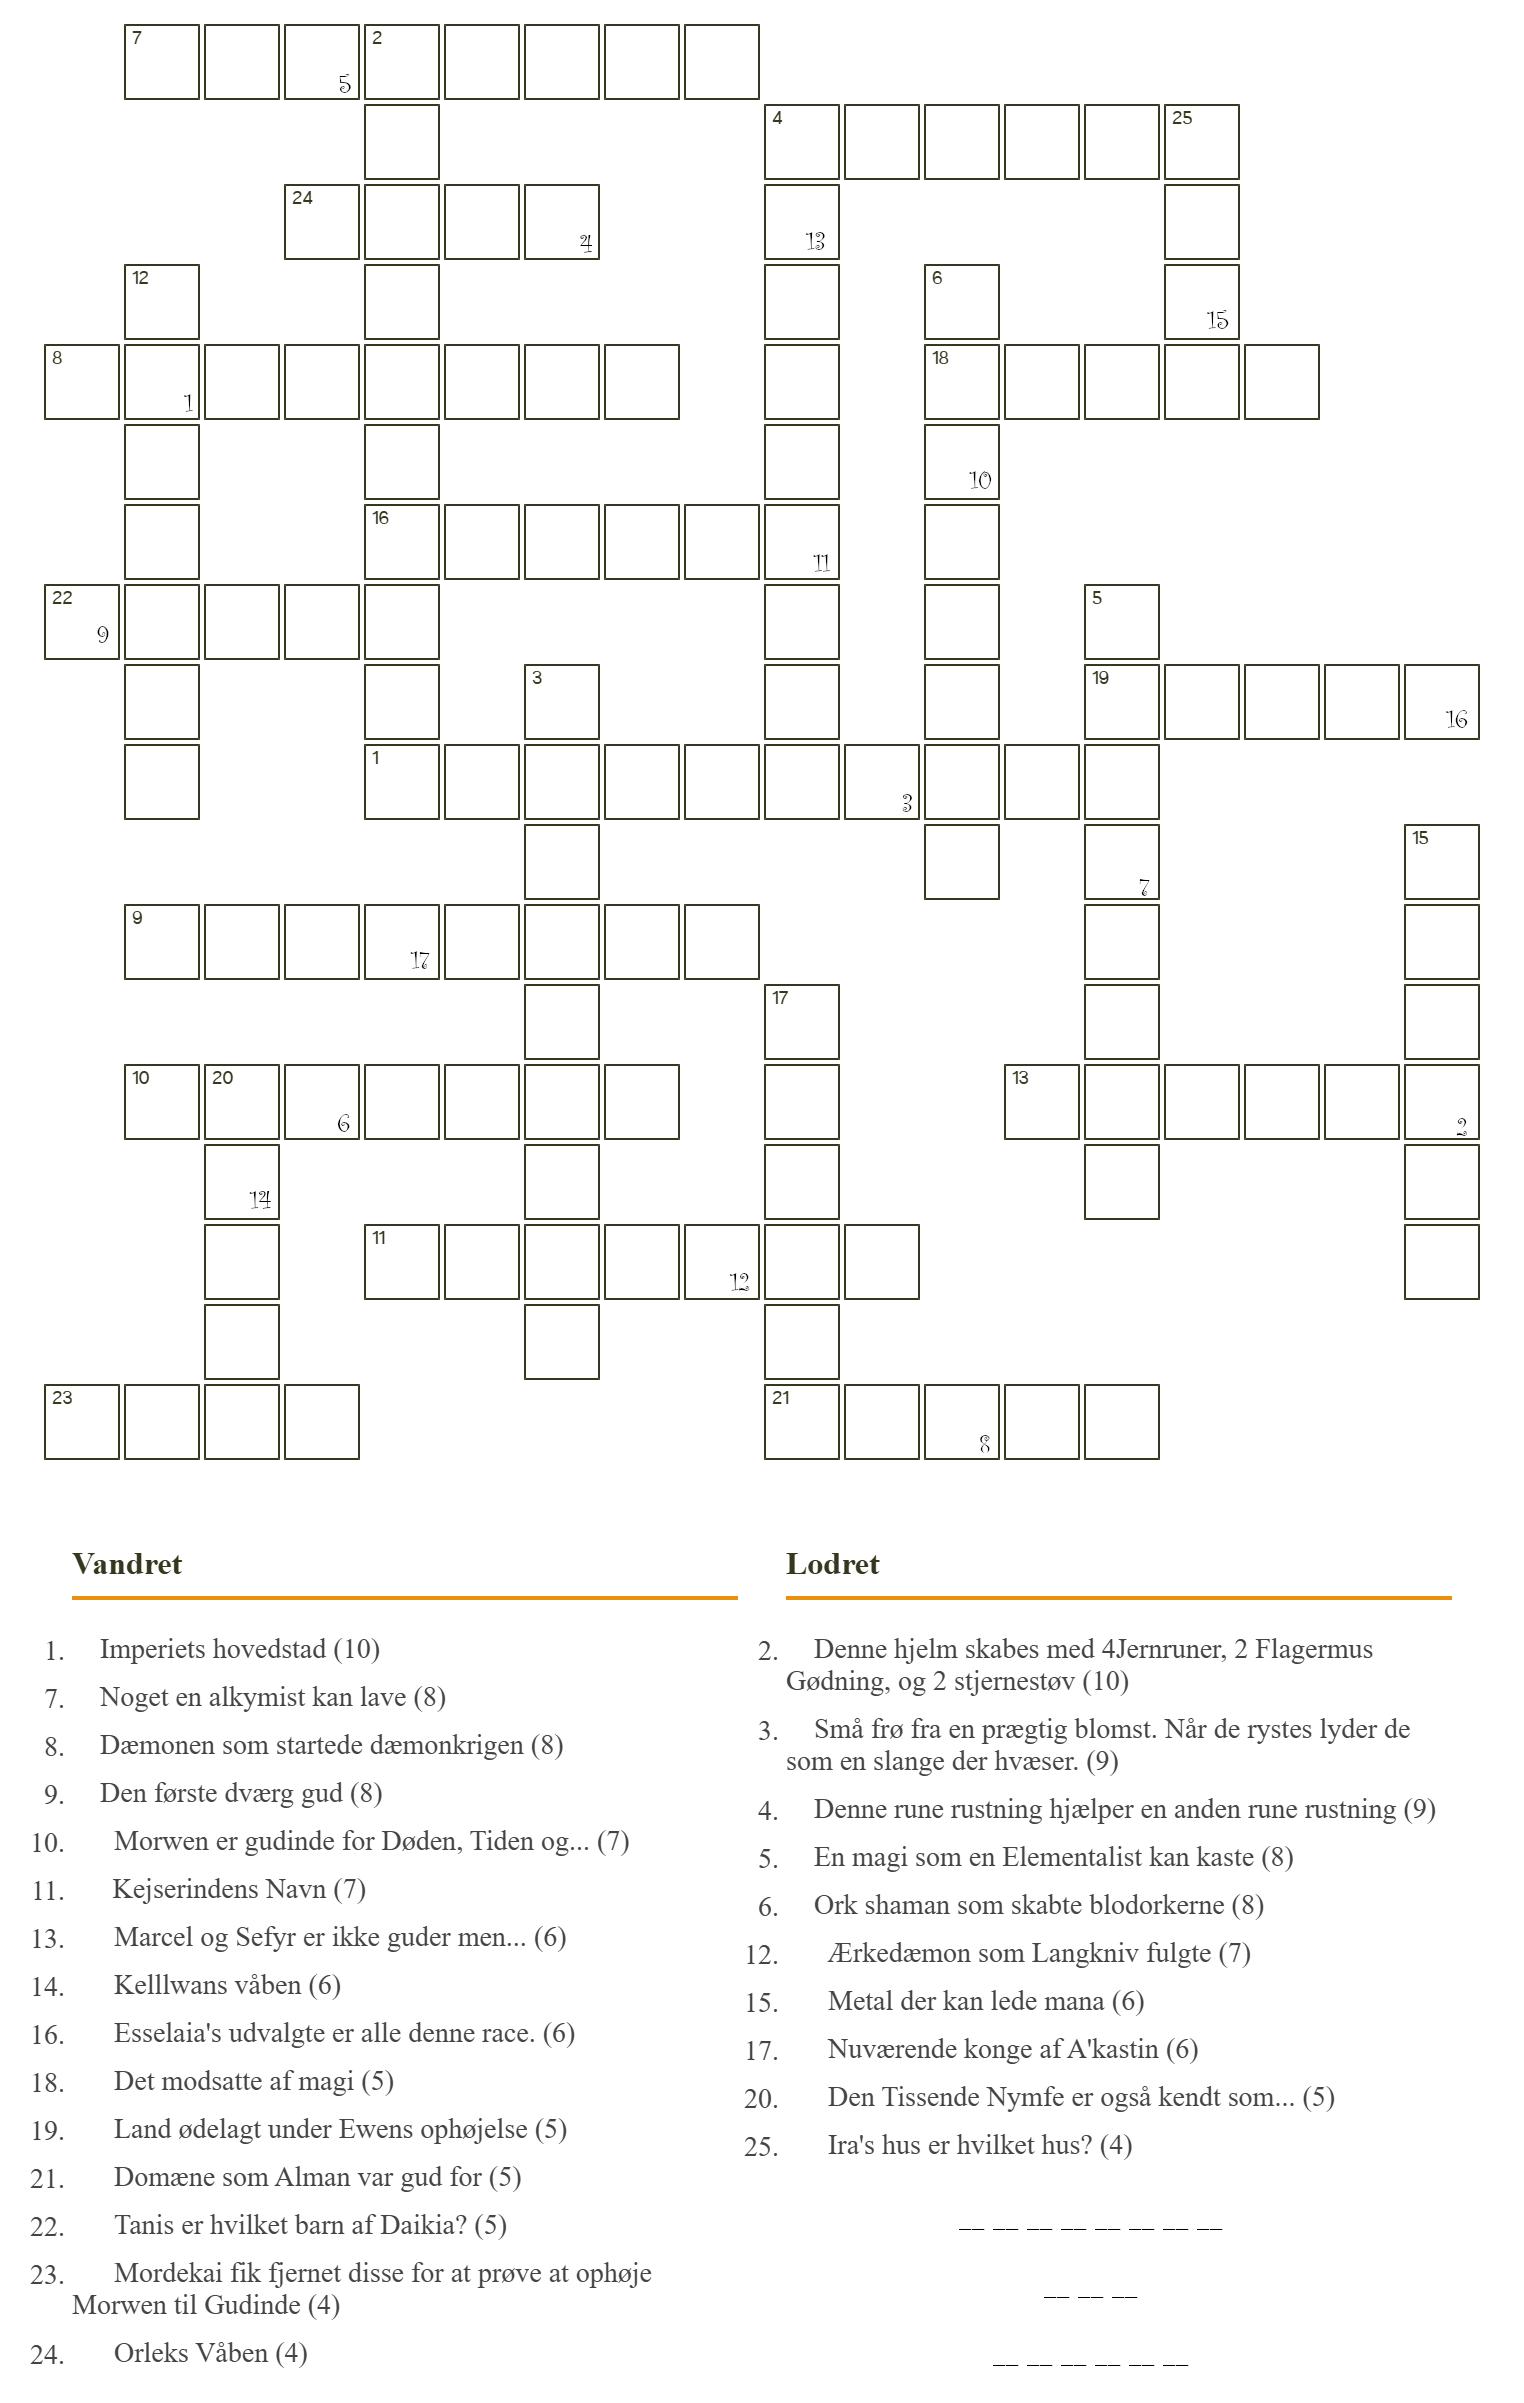
\includegraphics[width=\textwidth]{krydsord1-Blank.png}
\end{figure}

\section*{Reklamer}
\subsection*{BRING JERN! OG SULFUR!}
\begin{figure}[H]
  \centering
  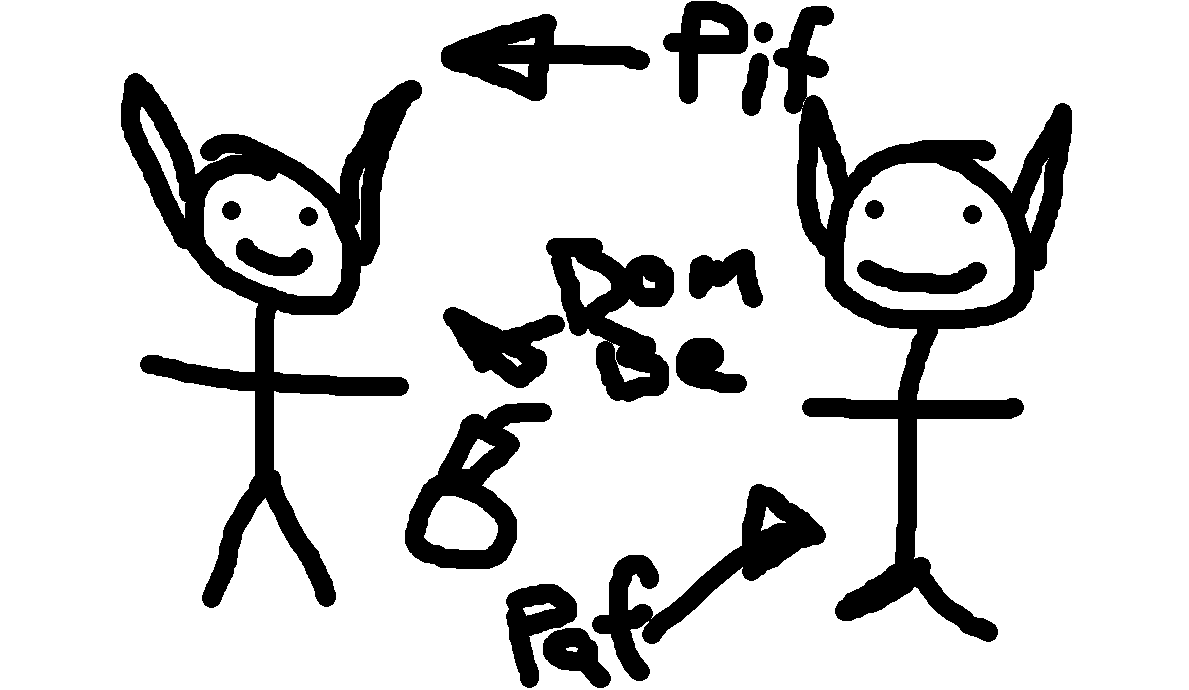
\includegraphics[width=0.9\textwidth]{PIFPAF.png}
\end{figure}
VI BRUG FOR SULFUR OG JERN TIL SPRINGE EVLER OP! DU BRING OS 5 JERN OG 5 SULFUR OG VI GIVE DIG SPECIEL PREMIE! DET VÆRE BOMBE I BREV! 
- PIF OG PAF!

\begin{center}
\fbox{
\begin{minipage}{0.9\linewidth}

\begin{center}
{\Large \textbf{KELLLWAN KIRKEN KALDER}}\
\medskip
{\large \textit{Sydporten skal genopbygges}}
\end{center}

\par\medskip

Efter år med fejlslagne forsøg er arbejdet ved Sydporten nu begyndt under Kelllwan Kirkens ledelse. Men sten rejser sig ikke alene, og dæmonerne fra Letho venter ikke tålmodigt.

\par\medskip

Kirken søger derfor arbejdere, minefolk, eventyrere og ærlige borgere til indsamling af materialer til rigets forsvar.

\par\medskip

\begin{center}
\textbf{BETALING UDBETALES DIREKTE AF KELLLWAN KIRKEN}
\end{center}

\begin{center}
\Huge
10 Fjend for Jern\\
20 Fjend for Mitril
\end{center}

\par\medskip

Materialer afleveres ved Kelllwan Kirkens lejre nær Sydporten.

\par\medskip

Kun gennem handling sikres Kalish mod Lethos rædsler.


\end{minipage}
}
\end{center}

\subsection*{Bliv rig uden at arbejde!}

Handelskompagniet giver dig en \textbf{eksklusiv mulighed} for at blive rig uden at løfte en finger! \\[0.5em]

Tjen op til \textbf{500 Fjend per dag}! \\[0.5em]

Alt du skal gøre, er at samle \textbf{Kongetand}! Handelskompagniet opkøber i øjeblikket alle de kongetand, vi kan få fat i. \\[0.5em]

Når du har bevist, at du kan samle 3 kongetand, får du \textbf{eksklusive rettigheder} til at oprette dit eget indsamlingskompagni! \\[1em]

\textit{Sådan fungerer det:}
\begin{itemize}
  \item Du samler 3 kongetander.
  \item Du finder 3 venner, der arbejder under dig.
  \item Hver af dem samler 3 kongetand til dig. Du har nu 9!
  \item Når de finder 3 venner hver, får du hele 36 kongetand!
\end{itemize}

Med vores atraktive handelsrate tilbyder vi \textbf{5 HKG}\footnote{Handelskompagni Guld} per kongetand. \\[0.5em]

Beviser du dit værd, bliver du udpeget til at være den officielle \textit{"Viceformand for eksklusiv kongetandsdistribution og indsamling"}.\footnote{Bevis for denne titel koster 5000 HKG eller 50 Fjend.} \\[1em]

\textbf{Kontakt din lokale repræsentant for Handelskompagniet i dag!}

\separator



\begin{center}
\fbox{%
\begin{minipage}{0.9\linewidth}
\centering
\vspace{2em}
\resizebox{\linewidth}{!}{%
\begin{tikzpicture}
\path[
  decorate,
  decoration={
    text along path,
    text={|\Large\bfseries|KOM SPIS VED DEN TISSENDE NYMFE},
    text align=center
  }
]
(-6,0) arc[start angle=160, end angle=20, radius=6cm];

\useasboundingbox (-6,0) rectangle (6,1.4);
\end{tikzpicture}%
}

\vspace{-0.5em}

{\LARGE\bfseries KOM OVER TIL KROEN!}

\begin{itemize}
  \item ØL: 1 Fjend
  \item Mad: 2 Fjend
  \item Flaske: 10 Fjend
  \item God Stemning: 0 Fjend
\end{itemize}

\end{minipage}%
}
\end{center}



\separator
% ====== Back matter (optional) ======
\section*{Kontakt}
Redaktionen, 1864 Salezstad

Ønsker du en artikel i Den Rullende Sten er det altid muligt at betale 15 Fjend for en 1 sides artikel.

\begin{figure}[H]
  \centering
  
\includegraphics[width=0.9\textwidth]{vinterkroneSkjold.png}
\end{figure}
Vi takker Familien Vinterkrone for deres støtte til Avisen.
\end{document}